\documentclass{article}
\usepackage{helvet}


\usepackage{cite}
\usepackage{amsmath,amssymb,amsfonts}
\usepackage{algorithmic}
\usepackage{graphicx}
\usepackage{textcomp}
\usepackage{xcolor}
\usepackage{hyperref}
\usepackage{placeins}
\usepackage{graphicx}
\usepackage{subcaption}
\usepackage{physics}




\def\BibTeX{{\rm B\kern-.05em{\sc i\kern-.025em b}\kern-.08em
    T\kern-.1667em\lower.7ex\hbox{E}\kern-.125emX}}


\title{Question 1: Assignment 3: CS 663, Fall 2024}
\author{
\IEEEauthorblockN{
    \begin{tabular}{cccc}
        \begin{minipage}[t]{0.23\textwidth}
            \centering
            Amitesh Shekhar\\
            IIT Bombay\\
            22b0014@iitb.ac.in
        \end{minipage} & 
        \begin{minipage}[t]{0.23\textwidth}
            \centering
            Anupam Rawat\\
            IIT Bombay\\
            22b3982@iitb.ac.in
        \end{minipage} & 
        \begin{minipage}[t]{0.23\textwidth}
            \centering
            Toshan Achintya Golla\\
            IIT Bombay\\
            22b2234@iitb.ac.in
        \end{minipage} \\
        \\ 
    \end{tabular}
}
}

\date{September 24, 2024}


\usepackage{amsmath}
\usepackage{amssymb}
\usepackage{fdsymbol}
\usepackage{bbding}
\usepackage{fontawesome}
\usepackage{pifont}
\usepackage{hyperref}
\usepackage{ulem,graphicx}
\usepackage[margin=0.5in]{geometry}

\begin{document}
\maketitle

\\

\begin{enumerate}
\item Consider the barbara256.png image from the homework folder. Implement the following in MATLAB: (a) an ideal low pass filter with cutoff frequency $D \in \{40, 80\}$, (b) a Gaussian low pass filter with $\sigma \in \{40,80\}$. Show the effect of these on the image, and display all filtered images in your report. Display the frequency response (in log absolute Fourier format) of all filters in your report as well. Comment on the differences in the outputs. Also display the log absolute Fourier transform of the original and filtered images. Comment on the differences in the outputs. Make sure you perform appropriate zero-padding while doing the filtering! \textsf{[15 points]}
\\
    \makebox[0pt][l]{\hspace{-7pt}\textit{Soln:}} % Aligns "Answer:" to the left
\\
\begin{figure}[!h]
    \centering
    \begin{minipage}{0.5\textwidth}
    \centering
    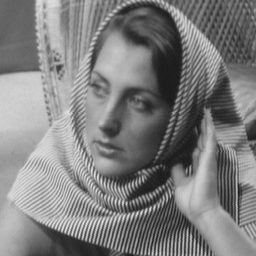
\includegraphics[width=0.4\linewidth]{HomeWork_3/Question_1/images/barbara256.png}
    \caption{barbara256.png original image}
    \end{minipage}%
    \hfill
    \begin{minipage}{0.5\textwidth}
    \centering
    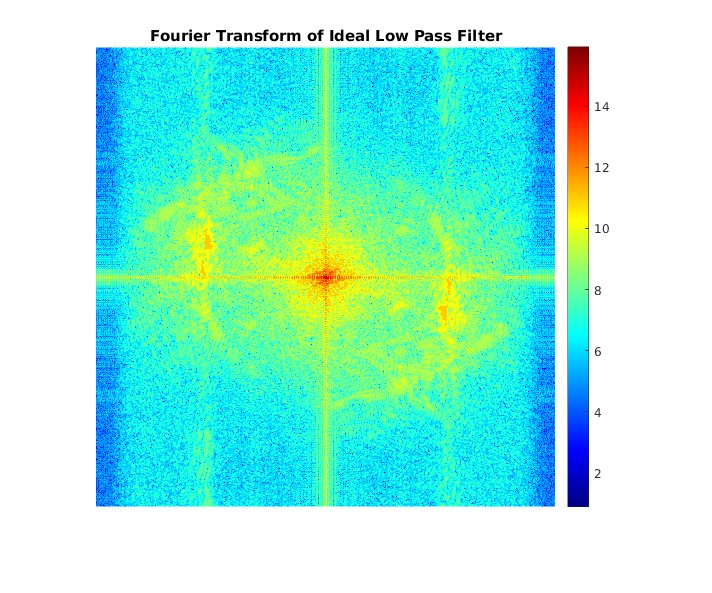
\includegraphics[width=0.5\linewidth]{HomeWork_3/Question_1/images/dtft_original.jpg}
    \caption{FFT of Original Image}
    \end{minipage}%
\end{figure}
\FloatBarrier
For the Ideal Low Pass Filter, D = 40, 60 and 80 are chosen and compared. Similariy for the Gaussian Low Pass Filter, $\sigma$ = 40, 60 and 80 are chosen and compared.

\subsection*{Ideal Low Pass Filter}
\begin{enumerate}
    \item Filtered Images
        \begin{figure}[!h]
            \centering
            \begin{minipage}{0.3\textwidth}
                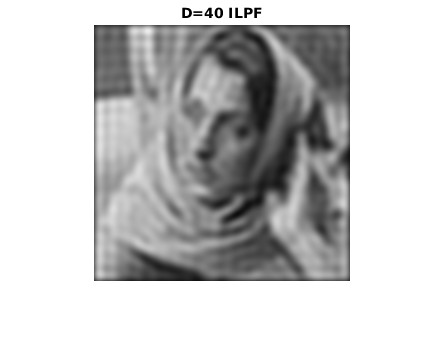
\includegraphics[width=1.2\textwidth]{HomeWork_3/Question_1/images/D=40/d40.jpg}
                \caption{D=40}
            \end{minipage}
            \hfill
                \centering
            \begin{minipage}{0.3\textwidth}
                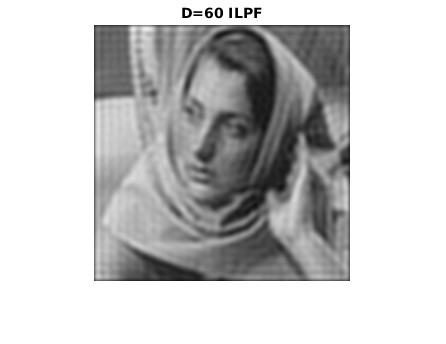
\includegraphics[width=1.2\textwidth]{HomeWork_3/Question_1/images/D=60/d60.jpg}
                \caption{D=60}
            \end{minipage}
            \hfill
                \centering
            \begin{minipage}{0.3\textwidth}
                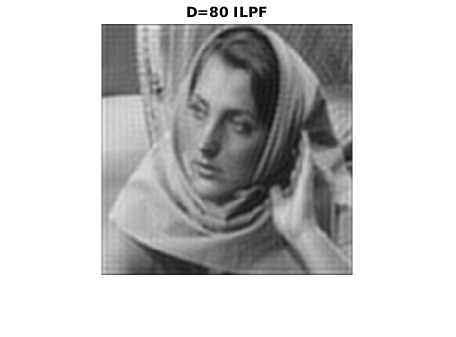
\includegraphics[width=1.2\textwidth]{HomeWork_3/Question_1/images/D=80/d80.jpg}
                \caption{D=80}
            \end{minipage}
            \hfill
        \end{figure}
        \newpage
    \item FFT of Filter
        \begin{figure}[!h]
            \centering
            \begin{minipage}{0.3\textwidth}
                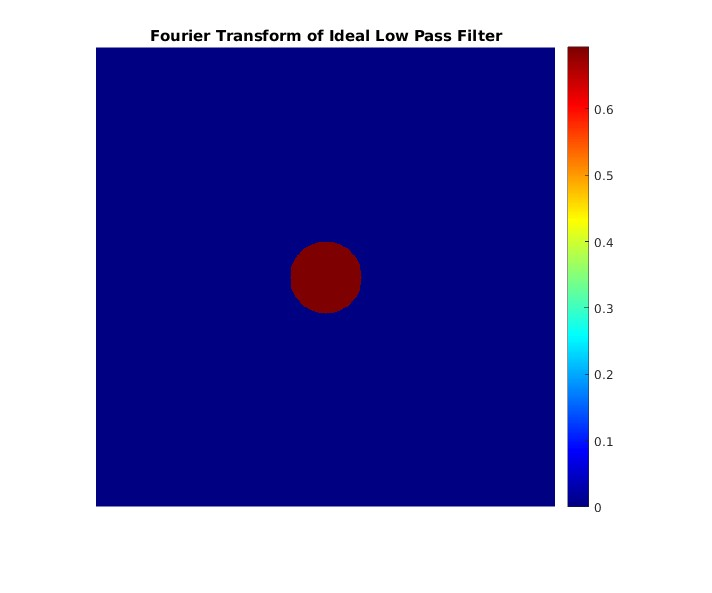
\includegraphics[width=1.2\textwidth]{HomeWork_3/Question_1/images/D=40/d40_filter.jpg}
                \caption{D=40}
            \end{minipage}
            \hfill
                \centering
            \begin{minipage}{0.3\textwidth}
                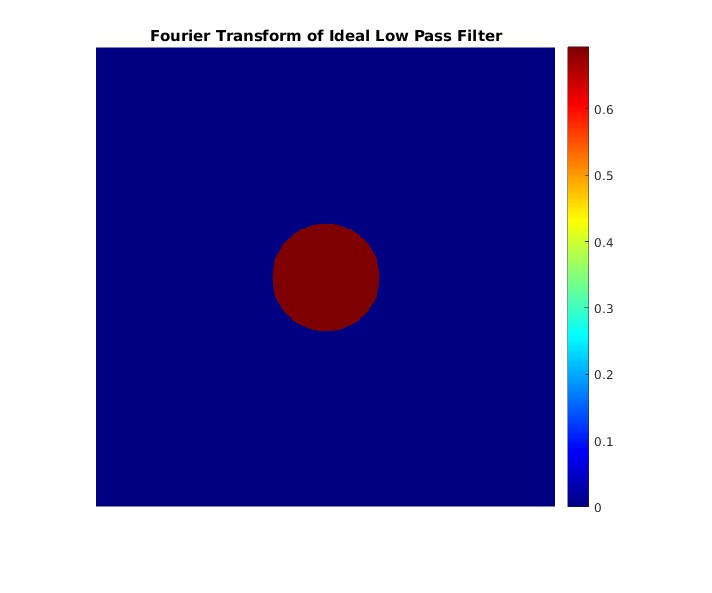
\includegraphics[width=1.2\textwidth]{HomeWork_3/Question_1/images/D=60/d60_filter.jpg}
                \caption{D=60}
            \end{minipage}
            \hfill
                \centering
            \begin{minipage}{0.3\textwidth}
                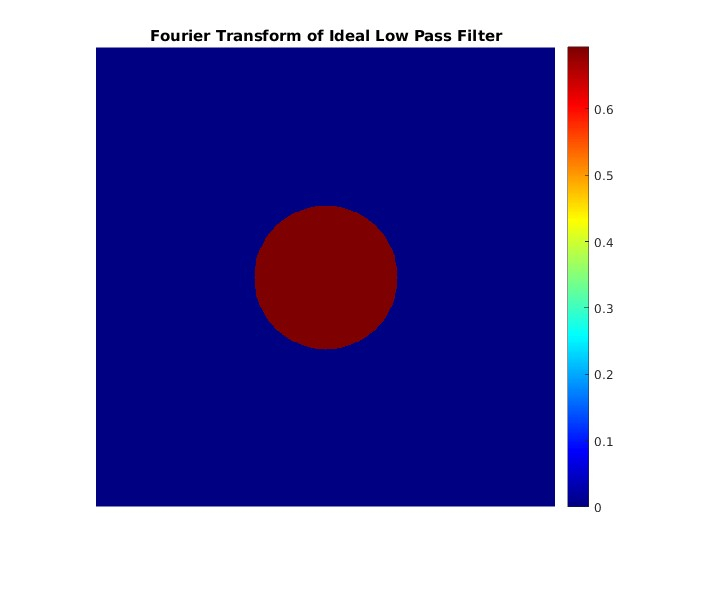
\includegraphics[width=1.2\textwidth]{HomeWork_3/Question_1/images/D=80/d80_filter.jpg}
                \caption{D=80}
            \end{minipage}
            \hfill
        \end{figure}
    \item FFT of Filtered Image
        \begin{figure}[!h]
            \centering
            \begin{minipage}{0.3\textwidth}
                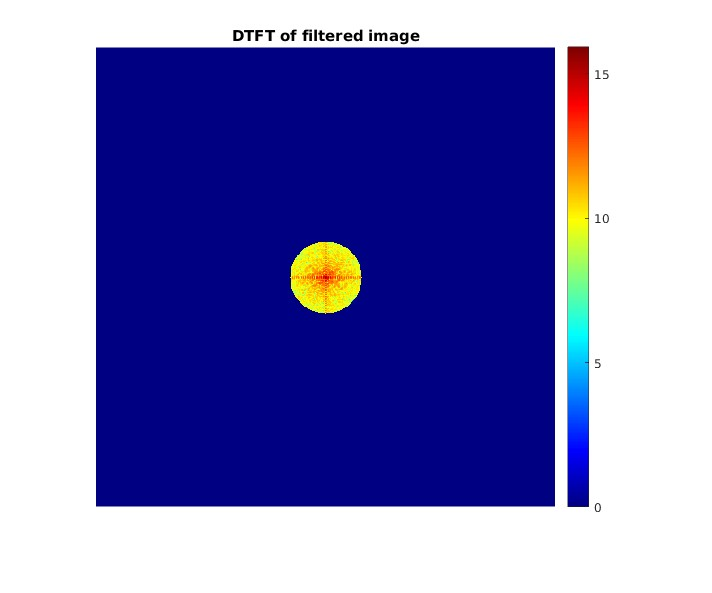
\includegraphics[width=1.2\textwidth]{HomeWork_3/Question_1/images/D=40/d_40_fourier.jpg}
                \caption{D=40}
            \end{minipage}
            \hfill
                \centering
            \begin{minipage}{0.3\textwidth}
                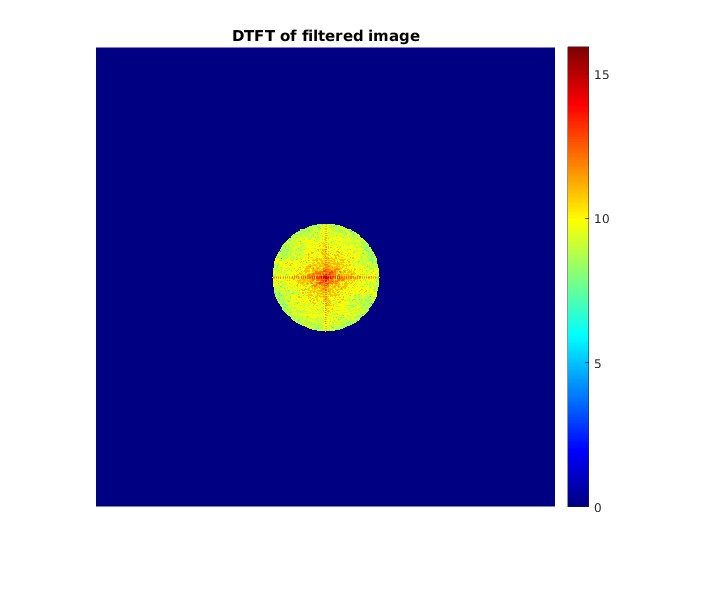
\includegraphics[width=1.2\textwidth]{HomeWork_3/Question_1/images/D=60/d60_fourier.jpg}
                \caption{D=60}
            \end{minipage}
            \hfill
                \centering
            \begin{minipage}{0.3\textwidth}
                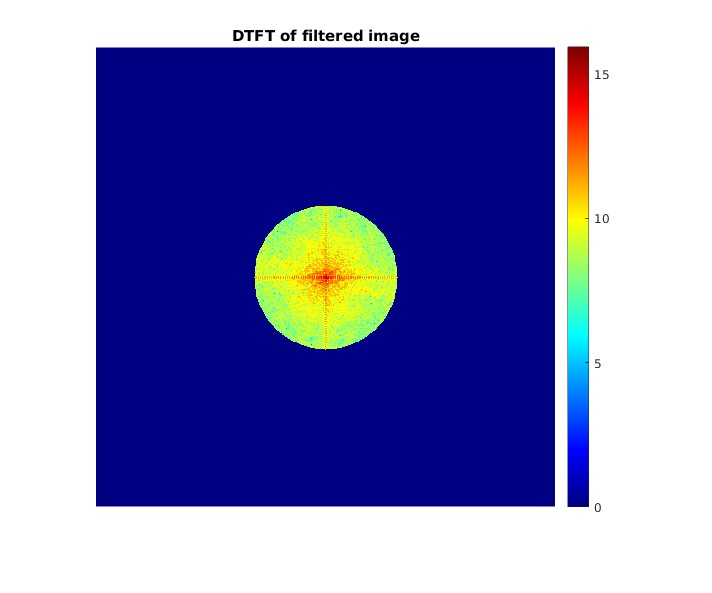
\includegraphics[width=1.2\textwidth]{HomeWork_3/Question_1/images/D=80/d80_fourier.jpg}
                \caption{D=80}
            \end{minipage}
            \hfill
        \end{figure}
\end{enumerate}

\subsection*{Gaussian Low Pass Filter}
\begin{enumerate}
    \item Filtered Images
        \begin{figure}[!h]
            \centering
            \begin{minipage}{0.3\textwidth}
                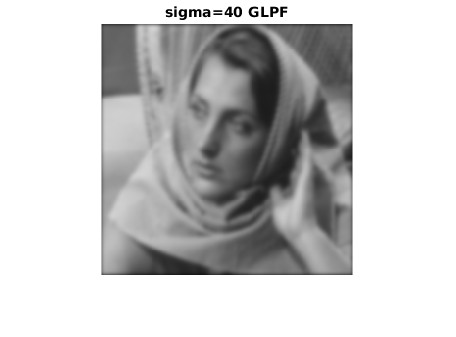
\includegraphics[width=1.2\textwidth]{HomeWork_3/Question_1/images/sigma=40/s40.jpg}
                \caption{$\sigma$ = 40}
            \end{minipage}
            \hfill
                \centering
            \begin{minipage}{0.3\textwidth}
                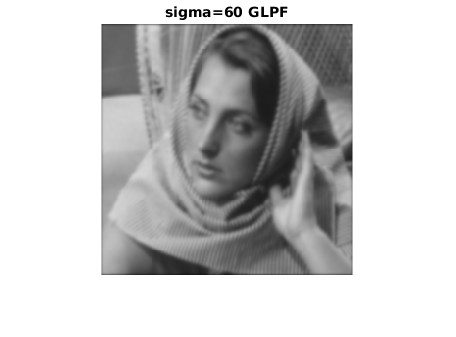
\includegraphics[width=1.2\textwidth]{HomeWork_3/Question_1/images/sigma=60/s60.jpg}
                \caption{$\sigma$ = 60}
            \end{minipage}
            \hfill
                \centering
            \begin{minipage}{0.3\textwidth}
                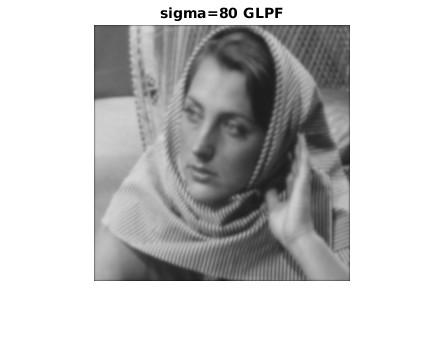
\includegraphics[width=1.2\textwidth]{HomeWork_3/Question_1/images/sigma=80/s80.jpg}
                \caption{$\sigma$ = 80}
            \end{minipage}
            \hfill
        \end{figure}
        \\\\\\
    \item FFT of Filter
        \begin{figure}[!h]
            \centering
            \begin{minipage}{0.3\textwidth}
                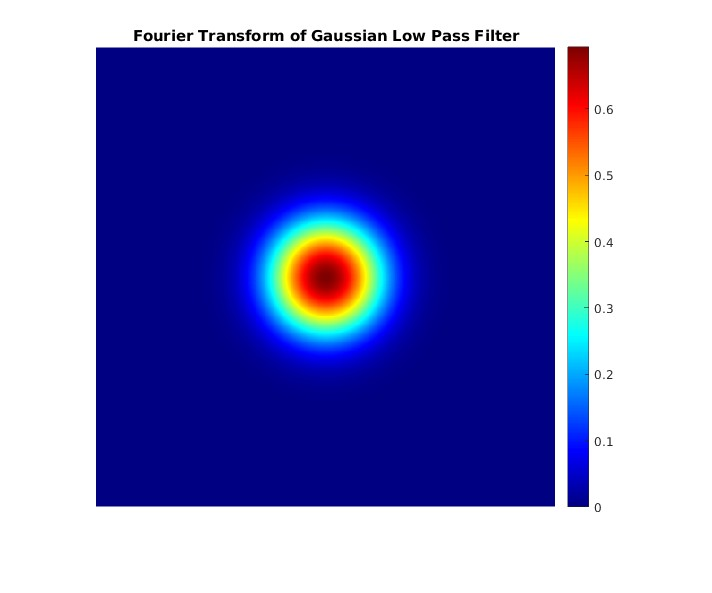
\includegraphics[width=1.2\textwidth]{HomeWork_3/Question_1/images/sigma=40/s40_filter.jpg}
                \caption{$\sigma$ = 40}
            \end{minipage}
            \hfill
                \centering
            \begin{minipage}{0.3\textwidth}
                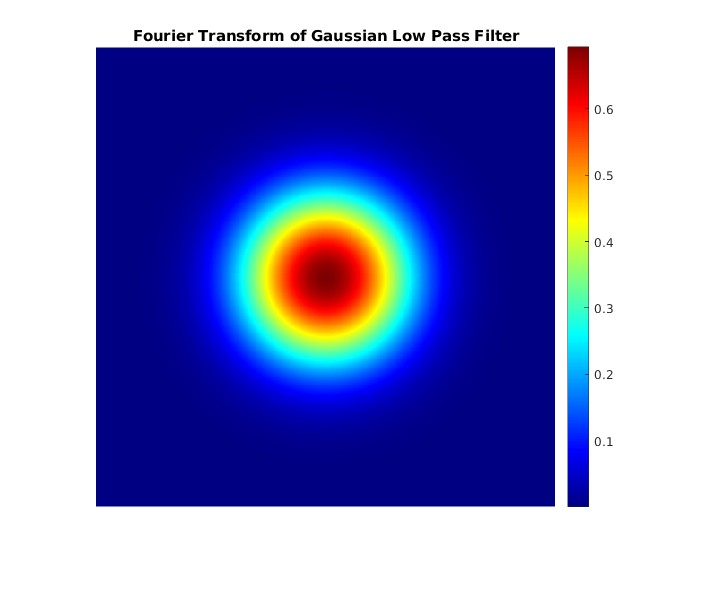
\includegraphics[width=1.2\textwidth]{HomeWork_3/Question_1/images/sigma=60/s60_filter.jpg}
                \caption{$\sigma$ = 60}
            \end{minipage}
            \hfill
                \centering
            \begin{minipage}{0.3\textwidth}
                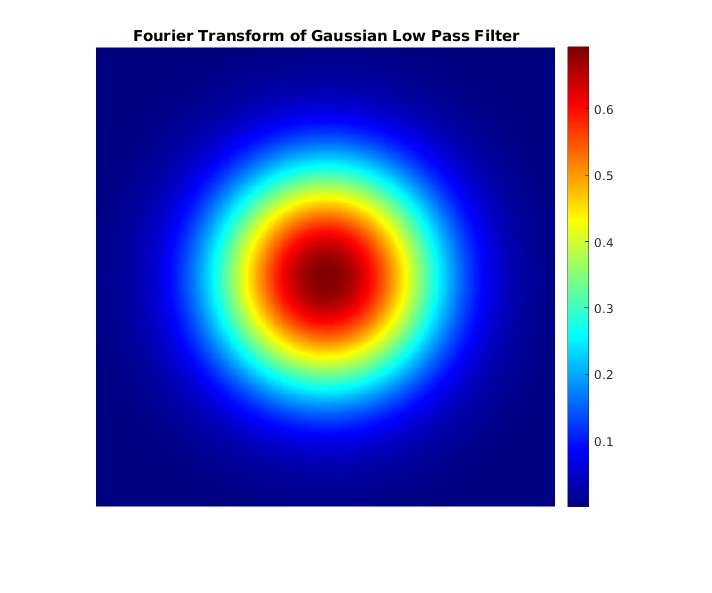
\includegraphics[width=1.2\textwidth]{HomeWork_3/Question_1/images/sigma=80/s80_filter.jpg}
                \caption{$\sigma$ = 80}
            \end{minipage}
            \hfill
        \end{figure}
    \FloatBarrier
    \item FFT of Filtered Images
        \begin{figure}[!h]
            \centering
            \begin{minipage}{0.3\textwidth}
                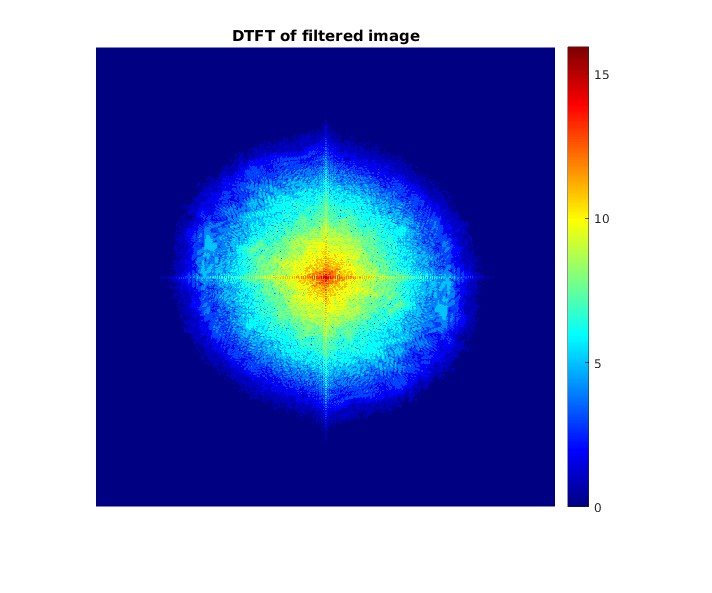
\includegraphics[width=1.2\textwidth]{HomeWork_3/Question_1/images/sigma=40/s40_fourier.jpg}
                \caption{$\sigma$ = 40}
            \end{minipage}
            \hfill
                \centering
            \begin{minipage}{0.3\textwidth}
                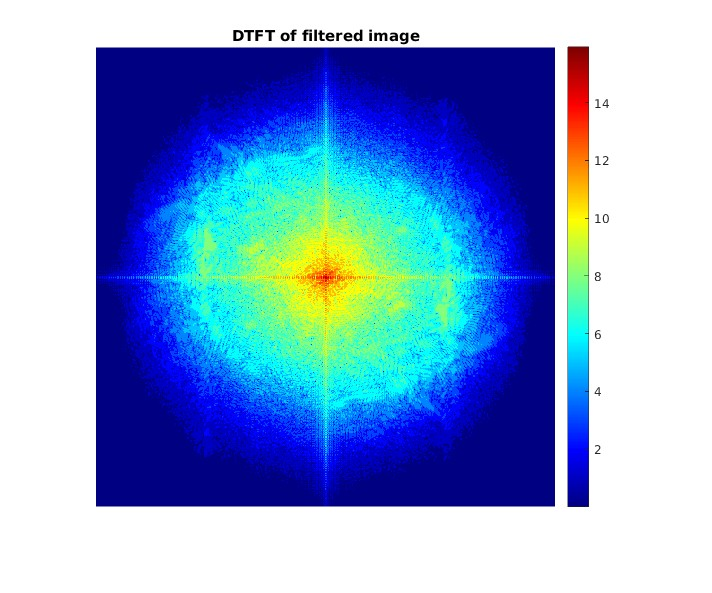
\includegraphics[width=1.2\textwidth]{HomeWork_3/Question_1/images/sigma=60/s60_fourier.jpg}
                \caption{$\sigma$ = 60}
            \end{minipage}
            \hfill
                \centering
            \begin{minipage}{0.3\textwidth}
                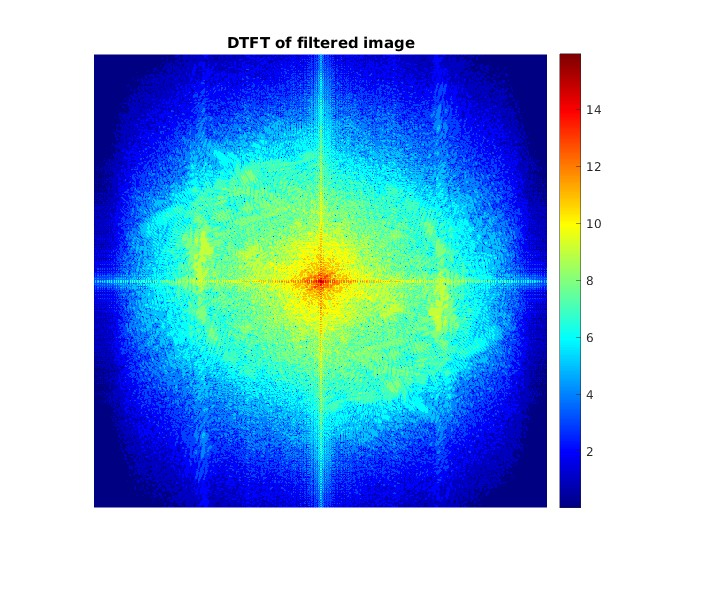
\includegraphics[width=1.2\textwidth]{HomeWork_3/Question_1/images/sigma=80/s80_fourier.jpg}
                \caption{$\sigma$ = 80}
            \end{minipage}
            \hfill
        \end{figure}

\end{enumerate}
\subsection*{Explanation}
Using an Ideal Low Pass filter, we introduce ringing-artifacts around the sharp-edges in the image due to jinc-function (3D-counterpart of sinc) function. In the spatial domain, the Ideal Low Pass thus causes blurring at the position of its central lobe and  the many smaller side-lobes give rise to "ringing". Also, we can see that as we increase D (cut-off frequency), the image becomes more clearer as the filter passes most of the significant harmonics of the original image. Hence, only noise/finer details are lost.\\
When we use a Gaussian Low Pass Filter instead, the ringing effect is not visible as here we are not completely eliminating the higher-frequencies but instead gradually weaken them. Hence, it is better to use this filter instead of Ideal Low Pass filter. Again, as $\sigma$ of the Gaussian filter is increased, the filtered image becomes more clear, owing to a higher spread of the Gaussian Lobe (in 3D).

\end{enumerate}
\end{document}
